% The Clever Algorithms Project: http://www.CleverAlgorithms.com
% (c) Copyright 2011 Jason Brownlee. Some Rights Reserved. 
% This work is licensed under a Creative Commons Attribution-Noncommercial-Share Alike 2.5 Australia License.

% Name
% The algorithm name defines the canonical name used to refer to the technique, in addition to common aliases, abbreviations, and acronyms. The name is used in terms of the heading and sub-headings of an algorithm description.
\section{Elastic Net} 
\label{sec:elasticnet}
\index{Elastic-Net}
\index{Na\"ive Elastic Net}
\index{Least Angle Regression Elastic Net}
\index{LARS-EN}

% other names
% What is the canonical name and common aliases for a technique?
% What are the common abbreviations and acronyms for a technique?
\emph{Elastic Net, Elasticnet, Elastic-Net, Na\"ive Elastic Net}

% Taxonomy: Lineage and locality
% The algorithm taxonomy defines where a techniques fits into the field, both the specific subfields of Computational Intelligence and Biologically Inspired Computation as well as the broader field of Artificial Intelligence. The taxonomy also provides a context for determining the relation- ships between algorithms. The taxonomy may be described in terms of a series of relationship statements or pictorially as a venn diagram or a graph with hierarchical structure.
\subsection{Taxonomy}
% To what fields of study does a technique belong?
Elastic Net is a Regularization method for Multiple Linear Regression models, and can be generalized to other machine learning methods.
An initial version was called the  Na\"ive Elastic Net, and the described algorithm is called Elastic Net.
% What are the closely related approaches to a technique?
It is related to other Regularization methods such as LASSO and Ridge Regression.

% Strategy: Problem solving plan
% The strategy is an abstract description of the computational model. The strategy describes the information processing actions a technique shall take in order to achieve an objective. The strategy provides a logical separation between a computational realization (procedure) and a analogous system (metaphor). A given problem solving strategy may be realized as one of a number specific algorithms or problem solving systems. The strategy description is textual using information processing and algorithmic terminology.
\subsection{Strategy}
% What is the information processing objective of a technique?
The information processing objective of the Elastic Net is to promote a parsimonious model.
% What is a techniques plan of action?
This is achieved by adding a penalty term that is a sum of the term used for Ridge Regression (squared sum of the coefficient values or $L_2$-norm) and the term used in the LASSO method (sum of absolute coefficient values or the $L_1$-norm). This penalty term is added to the models cost function with a penalty weight parameter ($\alpha$) and a shrinkage parameter $t$ that imposes a linear constraint on the term. 
It was proposed to address the limitations in the LASSO when Ridge Regression was demonstrated to perform better. 

Na\"ive Elastic Net is a two-stage procedure, first for each 

% optimization solutions
A modification of the Least Angle Regression (LARS) algorithm was proposed to solve the Elastic Net objective function called Least Angle Regression Elastic Net (LARS-EN).

% Heuristics: Usage guidelines
% The heuristics element describe the commonsense, best practice, and demonstrated rules for applying and configuring a parameterized algorithm. The heuristics relate to the technical details of the techniques procedure and data structures for general classes of application (neither specific implementations not specific problem instances). The heuristics are described textually, such as a series of guidelines in a bullet-point structure.
\subsection{Heuristics}
% What are the suggested configurations for a technique?
% What are the guidelines for the application of a technique to a problem instance?

\begin{itemize}
	\item It is expected to be useful in problems with a large number of predictors $p$ and a smaller number of observations $n$, $p>n$ problems.
	\item When the penalty weighting is 1 ($\alpha=1$), Na\"ive Elastic Net behaves like Ridge Regression. $\alpha$ is typically $\in \{0.1)$
	\item It can perform shrinkage of coefficients and variable selection simultaneously in the same way that the LASSO can.
	\item It has been demonstrated to outperform the LASSO while achieving a similarly sparse models.
	\item It encourages a grouping effect, where strongly correlated predictors tend to be in or out of the model together, a feature that had to be explicitly added to the LASSO in Group LASSO.
\end{itemize}

% sample script in R
\subsection{Code Listing}
% listing
Listing~\ref{glmnet_elastic_net} provides a code listing of the Elastic Net method in R.
% algorithm and package
The example uses the \texttt{glmnet()} function in the \texttt{glmnet} package. The demonstration provides an example of a logistic regression with regularization \cite{Friedman2011}. The \texttt{glmnet()} function provides efficient implementations of the LASSO method and Elastic Net for regression using the Cyclic Coordinate Descent algorithm in a path-wise fashion. For more information on the implemented algorithm details refer to Friedman et~al.\ \cite{Friedman2010}. For more information on this library type: \texttt{library(help="glmnet")}, and for more information on the function type: \texttt{?glmnet}.

% problem
The problem

The example shows...

Figure~\ref{plot:elastic_net_result} provides a plot of the coefficient values of each model for the given $t$ value.

\lstinputlisting[firstline=7,language=r,caption={Example of Elastic Net in R using the \texttt{glmnet()} function from the \texttt{glmnet} package.}, label=glmnet_elastic_net]{../src/algorithms/regularization/glmnet_elastic_net.R}

\begin{figure}[htp]
\centering
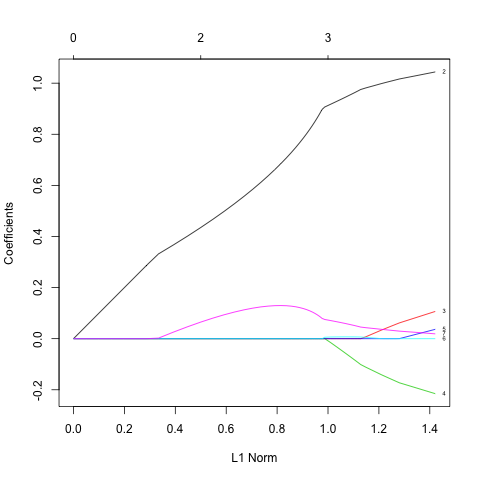
\includegraphics[scale=0.60]{a_regularization/elastic_net_result.png}
\caption{Graph of solution paths for Elastic Net.}
\label{plot:elastic_net_result}
\end{figure}

% other packages
% elasticnet package?


% References: Deeper understanding
% The references element description includes a listing of both primary sources of information about the technique as well as useful introductory sources for novices to gain a deeper understanding of the theory and application of the technique. The description consists of hand-selected reference material including books, peer reviewed conference papers, journal articles, and potentially websites. A bullet-pointed structure is suggested.
\subsection{References}
% What are the primary sources for a technique?
% What are the suggested reference sources for learning more about a technique?

% primary sources
\subsubsection{Primary Sources}
% seminal
The Elastic-Net was described by Zou and Hastie to address short-comings in LASSO by combining the penalty functions of Ridge Regression and the LASSO \cite{Zou2005}. Both a Na\"ive Elastic Net and the Elastic Net method proper were described as was a solution to the objective function called Least Angle Regression Elastic Net (LARS-EN).

% more info
\subsubsection{More Information}
% GLM
Friedman et~al.\ \cite{Friedman2010}

% cox model
Simon et~al.\ \cite{Simon2011}


% END
